\documentclass[border=10pt]{standalone}
\usepackage[T1]{fontenc}
\usepackage{tikz}
\usepackage[svgnames]{xcolor}
\usetikzlibrary{arrows.meta, positioning, calc, decorations.pathreplacing}

\colorlet{OrangeFill}{LightSalmon}
\colorlet{OrangeLine}{DarkSalmon!30!Chocolate}
\colorlet{GreenFill}{MediumAquamarine}
\colorlet{GreenLine}{MediumAquamarine!30!Teal}
\colorlet{PurpleFill}{MediumPurple}
\colorlet{PurpleLine}{MediumPurple!30!SlateBlue}
\colorlet{PinkFill}{Thistle}
\colorlet{PinkLine}{Thistle!30!Plum}
\colorlet{BlueFill}{LightSkyBlue}
\colorlet{BlueLine}{SteelBlue}
\colorlet{LimeFill}{YellowGreen}
\colorlet{LimeLine}{YellowGreen!30!Olive}
\colorlet{GrayFill}{LightGray!60!OldLace}
\colorlet{GrayLine}{RosyBrown!50!Silver}

\begin{document}
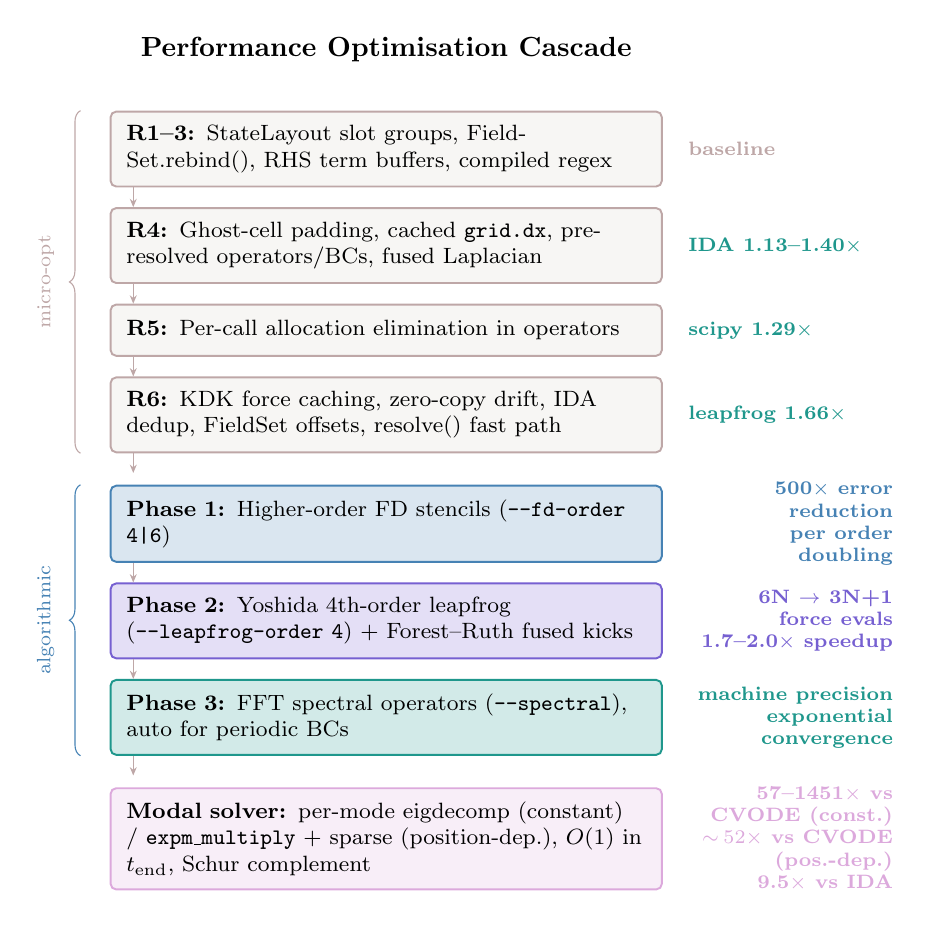
\begin{tikzpicture}[
    phase/.style={
        rectangle, rounded corners=2pt, minimum width=7.0cm,
        minimum height=0.65cm, draw=#1, line width=0.7pt,
        fill=#1!20, font=\footnotesize, align=left,
        text opacity=1, text=black, inner sep=5pt
    },
    phase/.default={black!60},
    speedup/.style={
        font=\scriptsize\bfseries, text=#1, align=right
    },
    speedup/.default={GreenLine},
    node distance=0.25cm
]

% Title
\node[font=\normalsize\bfseries] (title) at (0,0)
    {Performance Optimisation Cascade};

% --- Python micro-optimisation rounds ---
\node[phase=GrayLine, fill=GrayFill, fill opacity=0.3,
      below=0.5cm of title, text width=6.6cm] (r1)
    {\textbf{R1--3:} StateLayout slot groups, FieldSet.rebind(),
     RHS term buffers, compiled regex};
\node[speedup=GrayLine, right=0.2cm of r1.east, anchor=west]
    {baseline};

\node[phase=GrayLine, fill=GrayFill, fill opacity=0.3,
      below=of r1, text width=6.6cm] (r4)
    {\textbf{R4:} Ghost-cell padding, cached \texttt{grid.dx},
     pre-resolved operators/BCs, fused Laplacian};
\node[speedup=GreenLine, right=0.2cm of r4.east, anchor=west]
    {IDA 1.13--1.40$\times$};

\node[phase=GrayLine, fill=GrayFill, fill opacity=0.3,
      below=of r4, text width=6.6cm] (r5)
    {\textbf{R5:} Per-call allocation elimination in operators};
\node[speedup=GreenLine, right=0.2cm of r5.east, anchor=west]
    {scipy 1.29$\times$};

\node[phase=GrayLine, fill=GrayFill, fill opacity=0.3,
      below=of r5, text width=6.6cm] (r6)
    {\textbf{R6:} KDK force caching, zero-copy drift,
     IDA dedup, FieldSet offsets, resolve() fast path};
\node[speedup=GreenLine, right=0.2cm of r6.east, anchor=west]
    {leapfrog 1.66$\times$};

% --- Algorithmic phases ---
\node[phase=BlueLine, below=0.4cm of r6, text width=6.6cm] (p1)
    {\textbf{Phase 1:} Higher-order FD stencils
     (\texttt{--fd-order 4|6})};
\node[speedup=BlueLine, right=0.2cm of p1.east, anchor=west,
      text width=2.6cm]
    {500$\times$ error reduction\\per order doubling};

\node[phase=PurpleLine, below=of p1, text width=6.6cm] (p2)
    {\textbf{Phase 2:} Yoshida 4th-order leapfrog
     (\texttt{--leapfrog-order 4}) + Forest--Ruth fused kicks};
\node[speedup=PurpleLine, right=0.2cm of p2.east, anchor=west,
      text width=2.6cm]
    {6N $\to$ 3N+1 force evals\\1.7--2.0$\times$ speedup};

\node[phase=GreenLine, below=of p2, text width=6.6cm] (p3)
    {\textbf{Phase 3:} FFT spectral operators
     (\texttt{--spectral}), auto for periodic BCs};
\node[speedup=GreenLine, right=0.2cm of p3.east, anchor=west,
      text width=2.6cm]
    {machine precision\\exponential convergence};

% --- Modal solver ---
\node[phase=PinkLine, below=0.4cm of p3, text width=6.6cm] (modal)
    {\textbf{Modal solver:} per-mode eigdecomp (constant) /
     \texttt{expm\_multiply} + sparse (position-dep.),
     $O(1)$ in $t_{\mathrm{end}}$, Schur complement};
\node[speedup=PinkLine, right=0.2cm of modal.east, anchor=west,
      text width=2.6cm]
    {57--1451$\times$ vs CVODE (const.)\\
     $\sim\!52\times$ vs CVODE (pos.-dep.)\\
     9.5$\times$ vs IDA};

% Arrows (timeline)
\foreach \a/\b in {r1/r4, r4/r5, r5/r6, r6/p1, p1/p2, p2/p3, p3/modal} {
    \draw[-{Stealth[length=3pt, width=2.5pt]}, thin, GrayLine]
        (\a.south west) ++(0.3,0) -- ++(0,-0.25);
}

% Category braces
\draw[decorate, decoration={brace, amplitude=4pt, mirror, raise=2pt},
      GrayLine]
    ([xshift=-0.3cm]r1.north west) -- ([xshift=-0.3cm]r6.south west)
    node[midway, left=8pt, font=\scriptsize, text=GrayLine,
         align=right, rotate=90, anchor=south] {micro-opt};

\draw[decorate, decoration={brace, amplitude=4pt, mirror, raise=2pt},
      BlueLine]
    ([xshift=-0.3cm]p1.north west) -- ([xshift=-0.3cm]p3.south west)
    node[midway, left=8pt, font=\scriptsize, text=BlueLine,
         align=right, rotate=90, anchor=south] {algorithmic};

\end{tikzpicture}
\end{document}
